\documentclass{ximera}

\graphicspath{{./}{thePythagoreanTheorem/}{deMoivreSavesTheDay/}{complexNumbersFromDifferentAngles/}}

\usepackage{tikz}
\usepackage{tkz-euclide}
\usetkzobj{all}
\tikzstyle geometryDiagrams=[ultra thick,color=blue!50!black]
\newcommand{\tri}{\triangle}
\renewcommand{\l}{\ell}
\renewcommand{\P}{\mathcal{P}}
\newcommand{\R}{\mathbb{R}}
\newcommand{\Q}{\mathbb{Q}}

\newcommand{\Z}{\mathbb Z}

\renewcommand{\vec}{\mathbf}
\renewcommand{\d}{\,d}



%% Egyptian symbols

\usepackage{multido}
\newcommand{\egmil}[1]{\multido{\i=1+1}{#1}{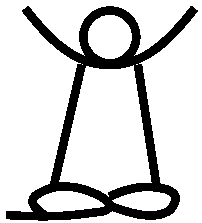
\includegraphics[scale=.1]{egyptian/egypt_person.pdf}\hspace{0.5mm}}}
\newcommand{\eghuntho}[1]{\multido{\i=1+1}{#1}{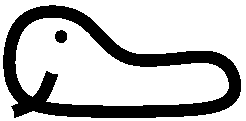
\includegraphics[scale=.1]{egyptian/egypt_fish.pdf}\hspace{0.5mm}}}
\newcommand{\egtentho}[1]{\multido{\i=1+1}{#1}{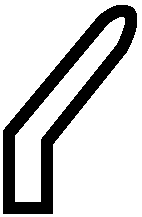
\includegraphics[scale=.1]{egyptian/egypt_finger.pdf}\hspace{0.5mm}}}
\newcommand{\egtho}[1]{\multido{\i=1+1}{#1}{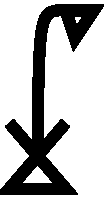
\includegraphics[scale=.1]{egyptian/egypt_lotus.pdf}\hspace{0.5mm}}}
\newcommand{\eghun}[1]{\multido{\i=1+1}{#1}{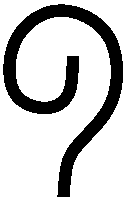
\includegraphics[scale=.1]{egyptian/egypt_scroll.pdf}\hspace{0.5mm}}}
\newcommand{\egten}[1]{\multido{\i=1+1}{#1}{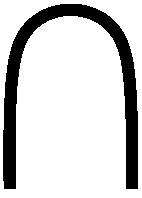
\includegraphics[scale=.1]{egyptian/egypt_heel.pdf}\hspace{0.5mm}}}
\newcommand{\egone}[1]{\multido{\i=1+1}{#1}{
\includegraphics[scale=.1]{egyptian/egypt_stroke.pdf}\hspace{0.5mm}}}
\newcommand{\egyptify}[7]{
 \multido{\i=1+1}{#1}{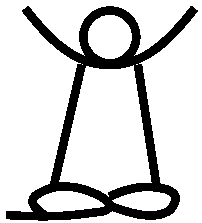
\includegraphics[scale=.1]{egyptian/egypt_person.pdf}\hspace{0.5mm}}
 \multido{\i=1+1}{#2}{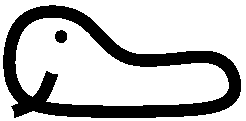
\includegraphics[scale=.1]{egyptian/egypt_fish.pdf}\hspace{0.5mm}}
 \multido{\i=1+1}{#3}{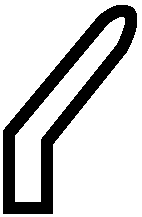
\includegraphics[scale=.1]{egyptian/egypt_finger.pdf}\hspace{0.5mm}}
 \multido{\i=1+1}{#4}{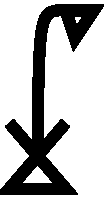
\includegraphics[scale=.1]{egyptian/egypt_lotus.pdf}\hspace{0.5mm}}
 \multido{\i=1+1}{#5}{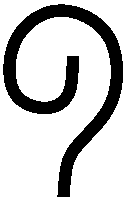
\includegraphics[scale=.1]{egyptian/egypt_scroll.pdf}\hspace{0.5mm}}
 \multido{\i=1+1}{#6}{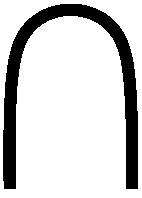
\includegraphics[scale=.1]{egyptian/egypt_heel.pdf}\hspace{0.5mm}}
 \multido{\i=1+1}{#7}{
\includegraphics[scale=.1]{egyptian/egypt_stroke.pdf}\hspace{0.5mm}}
 \hspace{.5mm}
}





\title{Heron's formula}
\begin{document}
\begin{abstract}
In this activity we will give two proofs of Heron's formula.
\end{abstract}
\maketitle


We'll start by giving a proof using synthetic geometry. 

\subsection*{Part I}

\begin{proposition}
The bisectors of the angles of a triangle meet at a point that is the center of the triangle's inscribed circle.
\end{proposition}

\begin{question}
How can we prove this?
\end{question}

\begin{question}
Now draw a triangle with vertices $A$, $B$, and $C$. Draw the incircle. Explain why the radii of the incircle touch the sides of the triangle at right angles. 
\end{question}

\begin{question}
Label the intersection of the radii with $D$ between $A$ and $B$, $E$ between $B$ and $C$, and $F$ between $C$ and $A$. Compute the areas of the following triangles:
\[
\triangle AOB,\qquad \triangle BOC,\qquad \triangle COA.
\]
Use this to express the area of $\triangle ABC$. 
\end{question}

\subsection*{Part II}

\begin{question}
Explain why
\[
\triangle AOD \cong \triangle AOF,\qquad
\triangle BOD \cong \triangle BOE,\qquad
\triangle COF \cong \triangle EOF.
\]
\end{question}


\begin{question}
If $AG \cong CE$, explain why $|BG|$ is the semiperimeter. 
\end{question}

\begin{question}
Find segments in your drawing equal to the length of 
\[
s-a,\qquad s-b,\qquad s-c.
\] 
\end{question}


\subsection*{Part III}

\begin{proposition}
If quadrilateral $AHBO$ has diagonals $AB$ and $OH$ with $\angle HAB$ and $\angle HOB$ being right angles, then $AHOB$ can be inscribed in a circle.
\end{proposition}

\begin{question}
Can you prove this proposition?
\end{question}

\begin{proposition}\label{P:cyclic}
The opposite angles of a cyclic quadrilateral sum to two right angles. 
\end{proposition}

\begin{question}
Can you prove this proposition?
\end{question}


\begin{question}
Now we need to decorate our triangle even more:
\begin{enumerate}
\item Draw $OL$ perpendicular to $OB$ cutting $AB$ at $K$. 
\item Draw $AM$ perpendicular to $OB$.
\item Call the intersection of $OL$ and $OM$, $H$. 
\item Draw $BH$. 
\end{enumerate}
Consider quadrilateral $AHBO$, explain why opposite angles sum to two right angles. 
\end{question}


\begin{question}
Explain why $\triangle COF$ is similar to $\triangle BHA$. Use this to explain why
\[
\frac{|AB|}{|AG|} = \frac{|AH|}{r}.
\]
\end{question}

\begin{question}
Explain why $\triangle KAH$ is similar to $\triangle KDO$. Use this to explain why
\[
\frac{|AK|}{|KD|} = \frac{|AH|}{r}.
\]
\end{question}

\begin{question}
Now we see 
\[
\frac{|AB|}{|AG|} = \frac{|AK|}{|KD|}.
\]
Add $1$ to both sides to obtain
\[
\frac{|BG|}{|AG|} = \frac{|AD|}{|KD|}.
\]
\end{question}


\begin{question}
Explain why $\triangle KDO$ is similar to $\triangle ODB$. Use this to explain why
\[
|KD|\cdot|BD| = r^2.
\]
\end{question}

\begin{question}
Multiply both sides of 
\[
\frac{|BG|}{|AG|} = \frac{|AD|}{|KD|}
\]
by $\frac{|BD|}{|BD|}$ to obtain
\[
r^2|BG|^2 = |AG|\cdot |BG|\cdot |AD|\cdot |BD|.
\]
\end{question}


\begin{question}
Explain how to deduce Heron's formula.
\end{question}


\subsection*{A modern proof}

\begin{question}
Now give a modern proof that a high school student might give. 
\end{question}

\begin{question}
Which proof was harder? Why didn't the ancient Greeks use our modern
proof?
\end{question}
\end{document}







